\documentclass[11pt, a4paper]{article}

\usepackage{graphicx}
\usepackage{verbatim}
\usepackage{color}

\setlength{\oddsidemargin}{0.0 cm}
\setlength{\evensidemargin}{0.0 cm}
\setlength{\topmargin}{0cm}
\setlength{\textheight}{23 cm}
\setlength{\textwidth}{16 cm}

\newcommand{\ttbar}{\mbox{t$\bar{\mathrm{t}}$}}

%\pagestyle{empty}

\setlength{\parindent}{0in}

\begin{document}

% -----------------------------------------------------
% title 
% -----------------------------------------------------

\begin{titlepage}

\begin{center}

\vspace{1.5cm}

{\Large Estimating contributions from different processes --} \\
\vspace{0.2cm}
{\Large A Bayesian approach to the template method}

\vspace{1.0cm}

{\Large Kevin Kr{\"o}ninger} 

\vspace{1.0cm}

{\Large II.~Institute of Physics} \\ 
\vspace{0.2cm}
{\Large University of G\"ottingen}

\end{center}

\vspace{1.0cm}

\begin{abstract}
In this note, the template method is reviewed and derived using Bayes'
Theorem. As an example, the estimation of the fraction of right-handed
W-bosons in top-decays is discussed. 
\end{abstract}

\end{titlepage}

% -----------------------------------------------------
% introduction 
% -----------------------------------------------------

\section{Introduction}
\label{section:introduction}

A common problem in HEP is to estimate the contributions from
different processes to an observed data set. A method often used is
the so-called {\it template method} where the data are given as a
histogram of a variable with maximal discrimination power between the
processes. In this note, the template method is explained and derived
using Bayes' Theorem. It is shown that efficiencies and systematic
uncertainties can be included in a natural way in this approach. As an
example, the estimation of the fraction of right-handed W-bosons in
top-decays is discussed. The technical implementation of method is
discussed in the last section.

% -----------------------------------------------------
% estimating contributions 
% -----------------------------------------------------

\section{Estimating contributions from different processes}
\label{section:estimation}

\subsection{Defining the problem} 

A set of $N$ events was measured. The events are known to come from a
number of different processes, $N_{\mathrm{p}}$. A process $i$
contributes with $N_{i}^{\mathrm{p}}$ events which is a random number
taken from a Poisson distribution with an expectation value
$\lambda_{i}^{\mathrm{p}}$. Neither $N_{i}^{\mathrm{p}}$ nor
$\lambda_{i}^{\mathrm{p}}$ are known\footnote{The case that prior
knowledge from, e.g., auxiliary measurements, is used will be
discussed separately.}. The aim of the study is to estimate the
expectation values of all processes involved.

\subsection{Modeling the problem} 

A variable $x$ is calculated for all events measured. The distribution
of $x$ is filled into a histogram which is divided into
$N_{\mathrm{b}}$ bins. The number of events in each bin is denoted by
$n_{i}$ and is assumed to fluctuate around an expectation value
$\lambda_{i}$. The fluctuations in each bin are assumed to be
independent. The expectation value for each bin can be calculated as
%
\begin{eqnarray}
\lambda_{i} = \sum_{j=1}^{N_{\mathrm{p}}} \, \lambda_{j}^{\mathrm{p}} \cdot \int_{\Delta x_{i}} f_{j}(x) \, dx \, , 
\label{eqn:expectation}
\end{eqnarray}
%
where $f_{j}(x)$ is the probability density of the variable $x$ for
process $j$ and normalized to unity. $\Delta x_{i}$ is the range of
the $i$th bin.

\subsection{Parameter estimation} 

The problem can be formulated in a Bayesian framework. The expectation
values, $\lambda_{i}^{\mathrm{p}}$, are the model parameters and the
set is denoted by $\vec{\lambda}^{\mathrm{p}}$ in the following. The
values of $x$ are the data and the data set is denoted by $\vec{x}$ in
the following. The {\it posterior probability density}, or {\it
posterior}, for the parameters given the data,
$p(\vec{\lambda}^{\mathrm{p}}|\vec{x})$, can be calculated using
Bayes' Theorem, i.e.,
%
\begin{eqnarray}
p(\vec{\lambda}^{\mathrm{p}}|\vec{x}) = \frac{p(\vec{x}|\vec{\lambda}^{\mathrm{p}}) \cdot p_{0}(\vec{\lambda}^{\mathrm{p}})}{\int p(\vec{x}|\vec{\lambda}^{\mathrm{p}}) \cdot p_{0}(\vec{\lambda}^{\mathrm{p}}) \, d\vec{\lambda}^{\mathrm{p}}} \, .
\label{eqn:bayes}
\end{eqnarray}
%
Here, $p(\vec{x}|\vec{\lambda}^{\mathrm{p}})$ is the probability for
observing $\vec{x}$ given $\vec{\lambda}^{\mathrm{p}}$, and sometimes
denoted {\it Likelihood}. The expression
$p_{0}(\vec{\lambda}^{\mathrm{p}})$ is the {\it prior probability
density}, or {\it prior}, and summarizes the knowledge about the
parameters $\vec{\lambda}^{\mathrm{p}}$ before the analysis of the
current data. In the present case, the Likelihood is defined as a
product of Poisson terms, i.e, the fluctuations in each bin are
assumed to be independent:
%
\begin{eqnarray*}
p(\vec{x}|\vec{\lambda}^{\mathrm{p}}) = \prod_{i=1}^{N_{\mathrm{b}}} \frac{\lambda_{i}^{n_{i}}}{n_{i}!} \cdot e^{-\lambda_{i}} \, .
\end{eqnarray*}

An estimator for the model parameters is the global mode, i.e., the
set of parameters, $\vec{\lambda}^{\mathrm{p}*}$, which maximizes the
posterior\footnote{Note that the sum of the estimated expectation
values does not have to be equal to the number of observed
events.}. An estimator for a single model parameter can be gained by
calculating the marginalized distribution of the posterior, i.e.,
%
\begin{eqnarray}
p(\lambda_{i}^{\mathrm{p}}|\vec{x}) = \int p(\vec{\lambda}^{\mathrm{p}}|\vec{x}) \prod
_{j \ne i}^{N_{p}} d\lambda_{j}^{\mathrm{p}} \, .
\end{eqnarray}
%
Typical estimators for $\lambda_{i}^{p}$ are the mode, mean and median
of the marginalized distribution\footnote{Note that the global mode
and the mode of the marginalized distributions do not have to be
equal.}. Uncertainties on the parameter can be obtained by
calculating, e.g., the 16\%-84\% quantiles of the distribution, the
RMS or the smallest interval containing 68\%. Similiarly, limits on a
single parameter can be obtained by solving the equation (for the 90\%
upper limit)
%
\begin{eqnarray}
0.9 = \int_{\lambda_{i, \mathrm{min}}^{\mathrm{p}}}^{\lambda_{i,
    \mathrm{90\%}}^{\mathrm{p}}} p(\lambda_{i}^{\mathrm{p}}|\vec{x})
\, d\lambda_{i}^{\mathrm{p}} \, 
\end{eqnarray}
%
for $\lambda_{i, \mathrm{90\%}}$.

\subsection{Templates} 

In most applications, the probability densities $f_{j}(x)$ are
estimated by frequency distributions taken from Monte Carlo which are
then referred to as {\it templates}. The statistical uncertainty on
these distributions are assumed to be negligible. If this assumption
is not valid, alternatives have to be considered, e.g., parameterizing
or smoothing the distribution, or using, e.g., kernel density
estimators. This is particularly important if a distribution has bins
with zero entries. 

\subsection{Choosing proper parameter ranges} 

The expectation values are constrained to be larger or equal to zero
and below a value larger than the number of observed events. In
Bayesian inference, these constraints can be modeled via the priors. A
bias in the estimated expectation values is visible for a contribution
close to zero since negative contributions are not allowed. This is
expected since the model fitted is not suited to describe the data
(due to the extra parameter). Two solutions are possible:
%
\begin{enumerate}
	\item The expectation value is treated as an observable, not as a
	model parameter. Thus, negative expectation values could be
	allowed. This is unphysical but removes the bias. Note that a direct
	estimation of the uncertainties and limits is not possible in this
	case. The observables need to be mapped onto {\it real} physical
	quantities in a second step. If, however, the mapping is done by
	cutting off the negative tail, the bias in the physical quantity
	reappears.
%
	\item Different models are fit to the data, starting with the
	simplest, i.e., the one with the fewest parameters. A
	goodness-of-fit test for each model is performed and the simplest
	model in agreement with the data is chosen. The expectation values
	for that model are estimated. Their estimate will not be biased. Not
	all possible contributions, e.g., a particular
	$\lambda_{i}^{\mathrm{p}}$, have to be included in this model.  In
	order to set a limit on $\lambda_{i}^{\mathrm{p}}$, the model is
	extended by this contribution and the limit obtained from the
	marginalized distribution can be quoted as a limit.
\end{enumerate}

\subsection{Including efficiencies} 

The efficiencies for the different processes, $\epsilon_{j}$, can
vary, e.g., due to the underlying kinematics and selection
criteria. In general, the efficiencies depend on the variable under
study, i.e., $\epsilon_{j}=\epsilon_{j}(x)$. Efficiencies can be
included by replacing
%
\begin{eqnarray*}
\lambda_{j}^{\mathrm{p}} \rightarrow \epsilon_{j} \cdot \lambda_{j}^{\mathrm{p}} \, 
\end{eqnarray*}

in eqn.~\ref{eqn:expectation}: 
%
\begin{eqnarray}
\lambda_{i} = \sum_{j=1}^{N_{\mathrm{p}}} \, \lambda_{j}^{\mathrm{p}} \cdot \int_{\Delta x_{i}} \epsilon_{j}(x) \cdot f_{j}(x) \, dx \, . 
\label{eqn:efficiency}
\end{eqnarray}
%
In the following, uncertainties in the efficiencies, $\Delta
\epsilon_{j}^{\mathrm{eff}}(x)$ are taken into account by introducing
nuisance parameters $\delta_{\epsilon_{j}}^{\mathrm{eff}}$ and their
priors, $p_{0}(\delta_{\epsilon_{j}}^{\mathrm{eff}})$, which are
Gaussian functions with a mean value of zero and a standard deviation
of one. The uncertainties on the efficiencies are assumed to be linear
functions of $\delta_{\epsilon_{j}}^{\mathrm{eff}}$, i.e.,
%
\begin{eqnarray*}
\epsilon_{j}(x, \, \delta_{\epsilon_{j}}^{\mathrm{eff}}) = \epsilon_{j}(x) \cdot + \delta_{\epsilon_{j}}^{\mathrm{eff}} \cdot \Delta \epsilon_{j}^{\mathrm{eff}}(x) \, .
\end{eqnarray*}
%
Note that the overall efficiency is constrained to be positive. \\

Equation~\ref{eqn:bayes} then becomes
%
\begin{eqnarray}
p(\vec{\lambda}^{\mathrm{p}}|\vec{x}) = \int \frac{p(\vec{x}|\vec{\lambda}^{\mathrm{p}},\vec{\delta}_{\epsilon}^{\mathrm{eff}}) \cdot p_{0}(\vec{\lambda}^{\mathrm{p}}) \cdot p_{0}(\vec{\delta}_{\epsilon}^{\mathrm{eff}})}{\int p(\vec{x}|\vec{\lambda}^{\mathrm{p}},\vec{\delta}_{\epsilon}^{\mathrm{eff}}) \cdot p_{0}(\vec{\lambda}^{\mathrm{p}}) \cdot p_{0}(\vec{\delta}_{\epsilon}^{\mathrm{eff}}) \, \, d\vec{\delta}_{\epsilon}^{\mathrm{eff}} d\vec{\lambda}^{\mathrm{p}}} \, \, d\vec{\delta}_{\epsilon} \, . 
\end{eqnarray}
%

\subsection{Including prior knowledge} 

Prior knowledge on the individual contributions can come from
auxiliary measurements or theoretical constraints. An example for the
former is the estimation of the background contribution. A constraint
could be a relation between several contributions, e.g., it is
possible that the total background to a process is known, e.g., from a
sideband measurement, but the composition of the background is not
known.

\subsection{Including systematic uncertainties}

Systematic uncertainties are treated as uncertainties on the
efficiency, $\Delta \epsilon_{j}^{\mathrm{syst}}(x)$, and modeled in
the same way: for each source of systematic uncertainty, a nuisance
parameter, $\delta_{j}^{\mathrm{syst}}$, is introduced. Its prior is
assumed to be a Gaussian with a mean value of zero and a standard
deviation of one. The uncertainties on the efficiencies are assumed to
be linear functions of $\delta_{j}^{\mathrm{syst}}$, i.e.,
eqn.~\ref{eqn:efficiency} becomes
%
\begin{eqnarray*}
\epsilon_{j}(x, \, \delta_{\epsilon_{j}}^{\mathrm{eff}}, \, \delta_{j}^{\mathrm{syst}}) = \epsilon_{j}^{\mathrm{eff}}(x) \cdot + \delta_{\epsilon_{j}}^{\mathrm{eff}} \cdot \Delta \epsilon_{j}^{\mathrm{eff}}(x) + \delta_{j}^{\mathrm{syst}} \cdot \Delta \epsilon_{j}^{\mathrm{syst}}(x) \, .
\label{eqn:syst}
\end{eqnarray*}
%
Note that the total efficiency has to be positive although $\Delta
\epsilon_{j}^{\mathrm{syst}}(x)$ can be negative. This is the case,
e.g., if the overall efficiency does not change but the shape of the
distribution under study alters.

\subsection{Systematic uncertainties due to the fitting procedure}

Several sources of systematic uncertainty arise due to the fitting
procedure itself. These are

\begin{itemize}
%
	\item the statistical fluctuations and/or smoothing bias from the
	templates; 
%
	\item badly modeled distributions or unknown contributions to the
	data. A hypothesis test can, but does not necessarily have to be
	sensitive to those contributions;
%
	\item the bin width for the variable under study;
%
  \item the treatment of systematic uncertainties and uncertainties of the efficiency;
%
	\item the choice of prior probabilities. 
%
\end{itemize}

\clearpage
\pagebreak

% -----------------------------------------------------
% estimating contributions 
% -----------------------------------------------------

\section{An example}
\label{section:example}

\subsection{A measurement of the W-helicity fractions in top-decays} 

The helicity fractions of the W-boson can be measured in semi-leptonic
top-decays. The three different contributions $\lambda_{0}$,
$\lambda_{-}$, $\lambda_{+}$ and the background,
$\lambda_{\mathrm{bkg}}$, are estimated from the distribution of the
lepton angle in the rest-frame of the W-boson, $\cos \theta^{*}$. The
{\it true} values used for this analysis are summarized in
tab.~\ref{tab:example}. The data are binned in 100~bins. \\

The overall signal and the background contributions are known from the
cross-section measurement. The efficiencies for the individual
contributions are estimated from Monte Carlo. Gaussian uncertainties
are assumed in both cases. Three different sources of systematic
uncertainty are considered here. The numbers used for the example are
summarized in tab.~\ref{tab:example}. \\

\begin{table}
\begin{center}
\caption{Parameters used for the creation of the data set and the
fit ranges. The prior knowledge on the number of signal and background
events comes from the cross-section measurement. The total number of
signal events, $\lambda_{0}+\lambda_{-}+\lambda{+}$, is constrained to
$7,000\pm100$ events. The efficiencies and their error estimates are
taken from Monte Carlo.}
\begin{tabular}{lllll}
\hline
Parameter                 & Parameter value       & Range              & Prior ($\mu$) & Prior ($\sigma$) \\ 
\hline
$\lambda_{0}$             & 4,900                 & $(0,\,8000)$       & - & - \\ 
$\lambda_{-}$             & 2,100                 & $(0,\,8000)$       & - & - \\ 
$\lambda_{+}$             & 0                     & $(0,\,8000)$       & - & - \\ 
$\lambda_{\mathrm{bkg}}$  & $1.30\cdot 10^{6}$    & $(1.29\cdot 10^{6},\, 1.31\cdot 10^{6})$ &  $1.30\cdot10^{6}$ & 2,000 \\ 
\hline
$\delta_{\epsilon_{\mathrm{sgn}}}^{\mathrm{eff}}$    & 0 & $(-5.0,\, 5.0)$ & 0 & 1 \\ 
$\delta_{\epsilon_{\mathrm{bkg}}}^{\mathrm{eff}}$    & 0 & $(-5.0,\, 5.0)$ & 0 & 1 \\ 
$\delta_{\epsilon_{\mathrm{sgn}}}^{\mathrm{syst 1}}$ & 0 & $(-5.0,\, 5.0)$ & 0 & 1 \\ 
$\delta_{\epsilon_{\mathrm{bkg}}}^{\mathrm{syst 1}}$ & 0 & $(-5.0,\, 5.0)$ & 0 & 1 \\ 
$\delta_{\epsilon_{\mathrm{sgn}}}^{\mathrm{syst 2}}$ & 0 & $(-5.0,\, 5.0)$ & 0 & 1 \\ 
$\delta_{\epsilon_{\mathrm{bkg}}}^{\mathrm{syst 2}}$ & 0 & $(-5.0,\, 5.0)$ & 0 & 1 \\ 
$\delta_{\epsilon_{\mathrm{sgn}}}^{\mathrm{syst 3}}$ & 0 & $(-5.0,\, 5.0)$ & 0 & 1 \\ 
$\delta_{\epsilon_{\mathrm{bkg}}}^{\mathrm{syst 3}}$ & 0 & $(-5.0,\, 5.0)$ & 0 & 1 \\ 
\hline
\end{tabular}
\end{center}
\label{tab:example}
\end{table}

The templates used for the generation of the data set and for the
analysis have the following form:
%
\begin{eqnarray*}
f_{0} & \propto & 1 - \cos \theta^{*\, 2} \, , \\
f_{-} & \propto & (1 - \cos \theta^{*})^{2} \, , \\
f_{+} & \propto & (1 + \cos \theta^{*})^{2} \, , \\
f_{\mathrm{bkg}} & \propto & \mathrm{const.} \, .
\end{eqnarray*}

The efficiencies and their uncertainties for the individual
contributions are parameterized as
%
\begin{eqnarray*}
\epsilon_{\mathrm{sgn}}^{\mathrm{eff}}(\cos \theta^{*}) & = & 0.15 + 0.05 \cdot (\cos \theta^{*}+1)\, , \\ 
\epsilon_{\mathrm{bkg}}^{\mathrm{eff}}(\cos \theta^{*}) & = & 0.001\, , \\ 
\Delta \epsilon_{\mathrm{sgn}}^{\mathrm{eff}}(\cos \theta^{*}) & = & 0.025\cdot(\cos \theta^{*} + 1)\, , \\
\Delta \epsilon_{\mathrm{bkg}}^{\mathrm{eff}}(\cos \theta^{*}) & = & 0.0005\, .
\end{eqnarray*}

The systematic uncertainties are parameterized in the following way 
% 
\begin{eqnarray*}
\Delta \epsilon_{\mathrm{sgn}}^{\mathrm{syst 1}}(\cos \theta^{*}) & = & 0.02 \, , \\
\Delta \epsilon_{\mathrm{bkg}}^{\mathrm{syst 1}}(\cos \theta^{*}) & = & 0.005 \, , \\
\Delta \epsilon_{\mathrm{sgn}}^{\mathrm{syst 2}}(\cos \theta^{*}) & = & 0.005\cdot(\cos \theta^{*} + 1) \, , \\
\Delta \epsilon_{\mathrm{bkg}}^{\mathrm{syst 2}}(\cos \theta^{*}) & = & 0.0005\cdot(\cos \theta^{*} + 1) \, , \\
\Delta \epsilon_{\mathrm{sgn}}^{\mathrm{syst 3}}(\cos \theta^{*}) & = & 0.02 -  0.0025 \cdot(\cos \theta^{*} + 1)^{2} \, , \\
\Delta \epsilon_{\mathrm{bkg}}^{\mathrm{syst 3}}(\cos \theta^{*}) & = & 0.001 - 0.00025 \cdot (\cos \theta^{*} + 1)^{2} \, . 
\end{eqnarray*}

As an example, fig.~\ref{fig:tempexample} shows the template for
$f_{+}$ signal contribution and the individual uncertainties. 

\begin{figure}
\begin{center}
%\includegraphics[width=0.8\textwidth]{./fig/.eps}
\caption{Left: Template for the $f_{+}$ signal contribution with two
 error bands (dark: systematic uncertainties alone, light: uncertainty
 on the efficiency and the systematic uncertainty). Right:
 Uncertainties of the efficiency and the systematics as a function of
 $\cos \theta^{*}$.}
\label{fig:tempexample}
\end{center}
\end{figure}

\clearpage
\pagebreak

\begin{comment}
\subsection{Estimating efficiencies and interpreting the expectation values}

The selection criteria in a real data analysis include a requirement
for a single high-$p_{T}$ electron or muon. I cannot take into account
if the electron or muon comes from the secondary decay of a tau. The
number of, e.g., selected electron events for a helicity state $h$,
$N_{e}^{\mathrm{sel},\, h}$, is thus
%
\begin{eqnarray*}
N_{e}^{\mathrm{sel},\, h} = N_{e}^{\mathrm{gen},\, h} \cdot \epsilon_{e} + N_{\tau}^{\mathrm{gen},\, h} \cdot \mathrm{BR}(\tau \rightarrow e) \cdot \epsilon'_{e} \, ,
\end{eqnarray*}
%
where $\mathrm{BR}(\tau \rightarrow e)$ is the branching ratio for the
decay $\tau \rightarrow e$ and $\epsilon'_{e}$ is the probability to
observe electron events from $\tau$-decays. Due to the different
kinematics, the efficiencies might differ. They are assumed to be the
equal in the following. The efficiency is estimated by solving the
equation for $\epsilon_{e}$. \\

For the same reason, the estimated expectation values are
%
\begin{eqnarray*}
\lambda_{e}^{\mathrm{tot}, h} & = & \lambda_{e}^{h} + \lambda_{\tau}^{, h} \cdot \mathrm{BR}(\tau \rightarrow e) \\ 
														  & \approx & \lambda_{e}^{h} \cdot (1 + \mathrm{BR}(\tau \rightarrow e)) \\ 
															& \approx & \lambda_{e}^{h} \cdot 1.178 \, . 
\end{eqnarray*}
%
This effect is neglected for the present example. 
\end{comment}

\subsection{Results}

Figure~\ref{fig:stack} shows the measured data and the estimated
contributions to the data including an error band. The $\chi^{2}$ for
each bin is shown in the bottom. The data is consistent with
$\lambda_{+}=0$. The overall $\chi^{2}/ndf$ is 85.8/92 corresponding
to a $\chi^{2}$-probability of 66.2\% for $100-2\cdot4=92$ degrees of
freedom. The Kolmogorov-Smirnov-probability is 99.9\%. The best fit
parameters (i.e., the global mode or the limit) are
%
\begin{eqnarray*}
\lambda_{0}^{*}            & = & 4856 \pm 846.4 \, , \\
\lambda_{-}^{*}            & = & 2139 \pm  \, 343, \\
\lambda_{+}^{*}            & < & \phantom{0}843.2 \mathrm{~(95\%~prob.)} \, , \\
\lambda_{\mathrm{bkg}}^{*} & = & 1.3\cdot10^{6} \pm 2\cdot10^{3} \, .
\end{eqnarray*} 

Figure~\ref{fig:marg} shows the marginalized distributions of the
parameters $\lambda_{+}$ (left) and $\lambda_{-}$
vs. $\lambda_{\mathrm{bkg}}$ as an example. The figure include a
comparison between the prior and the posterior distribution. An upper
limit of 843.2 events (for 95\% probability) can be set on
$\lambda^{+}$. The full error propagation yields a limit on the
fraction of
$f^{+}=\frac{\lambda_{+}}{\lambda_{0}+\lambda_{-}+\lambda_{+}}<11.98\%$. If
the constraint of positive expectation values is dropped, the
extracted fraction is $f^{+}=-0.014^{+0.067}_{-0.075}$.\\

\begin{figure}
\begin{center}
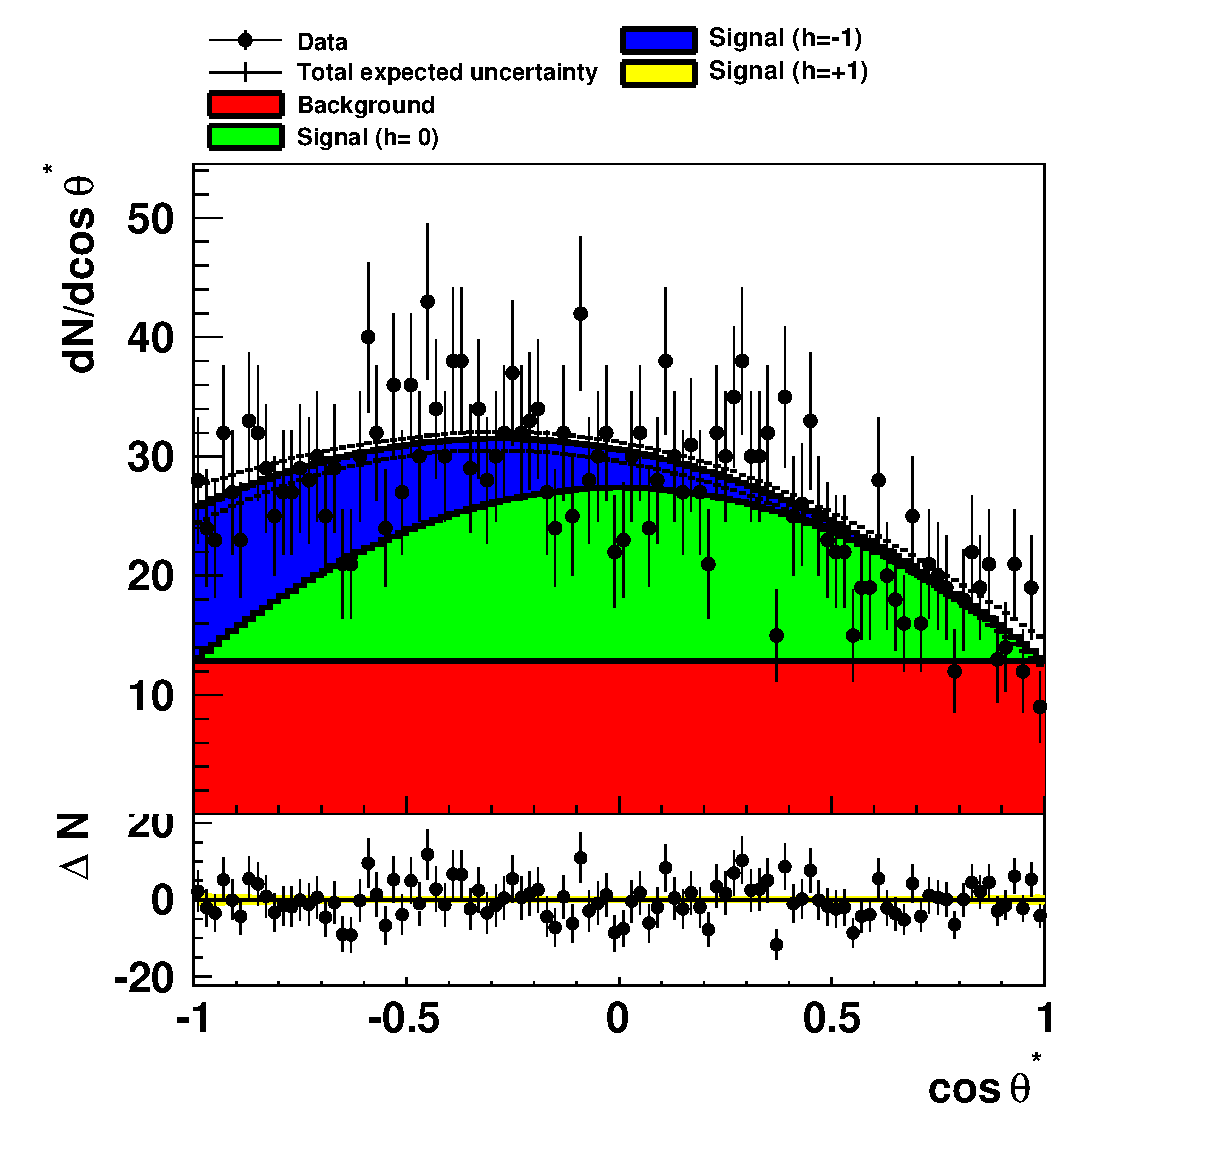
\includegraphics[width=0.8\textwidth]{./fig/model_stack.eps}
\caption{Distribution of the measured $\cos \theta^{*}$ value
(marker) and all distributions scaled to the best-fit parameters
(colored histograms). The bottom figure shows the difference between
the data and the scaled distributions (black marker) together with the
Poisson uncertainties (error bars) and the uncertainty on the scaled
distributions (yellow band) as a function of $\cos
\theta^{*}$.}
\label{fig:stack}
\end{center}
\end{figure}

\begin{figure}
\begin{center}
\begin{tabular}{cc}
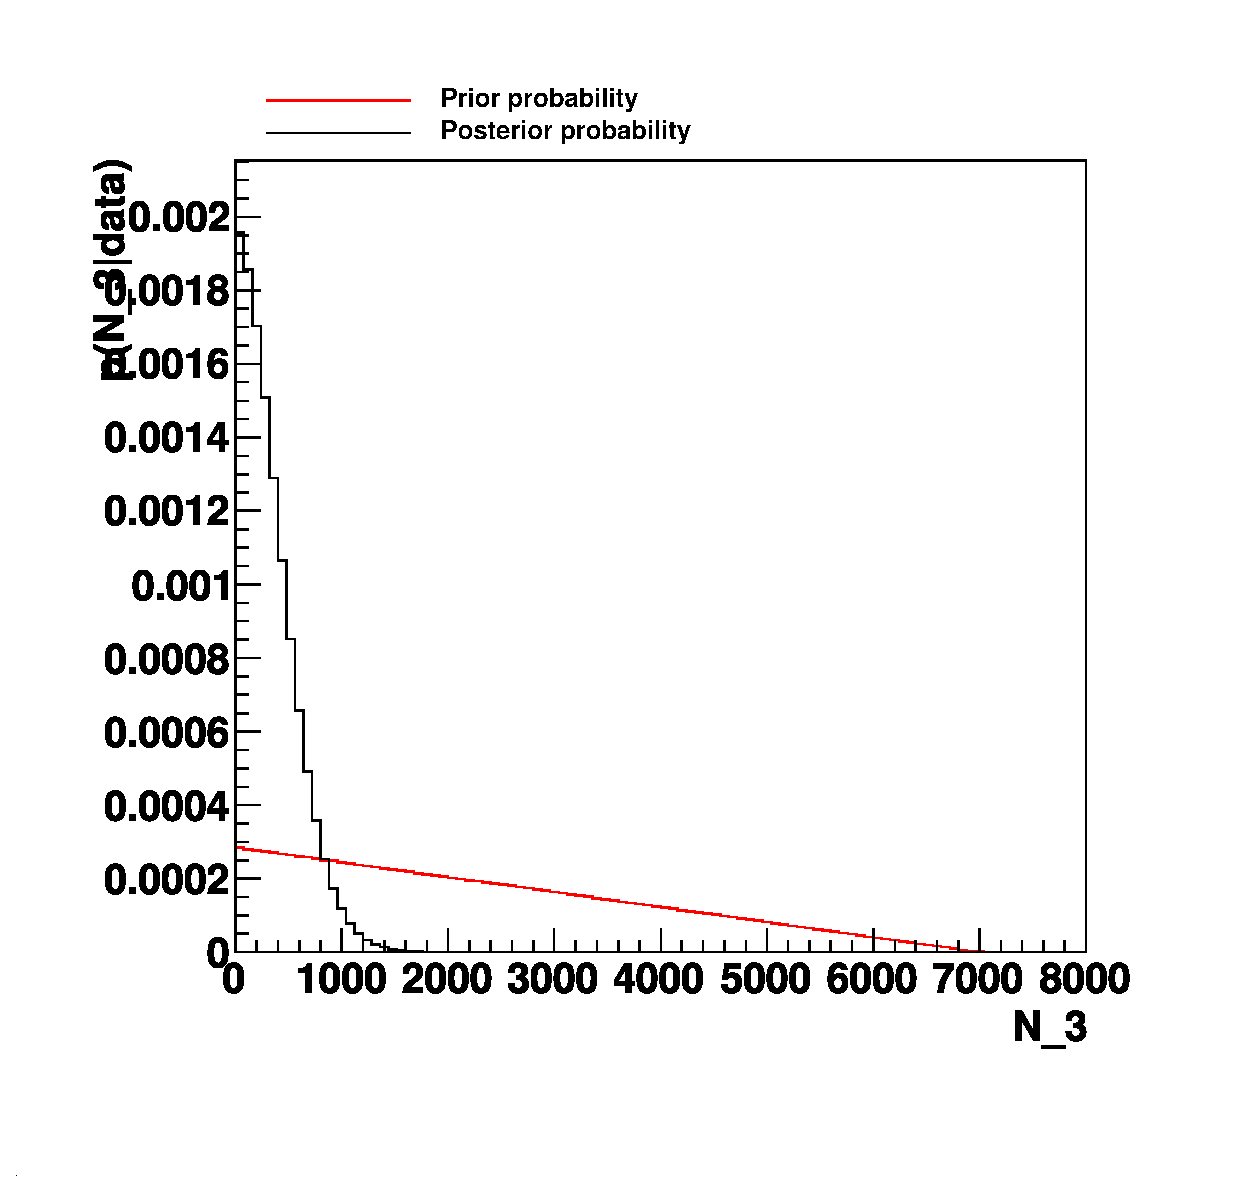
\includegraphics[width=0.45\textwidth]{./fig/lambda_fplus.eps} & 
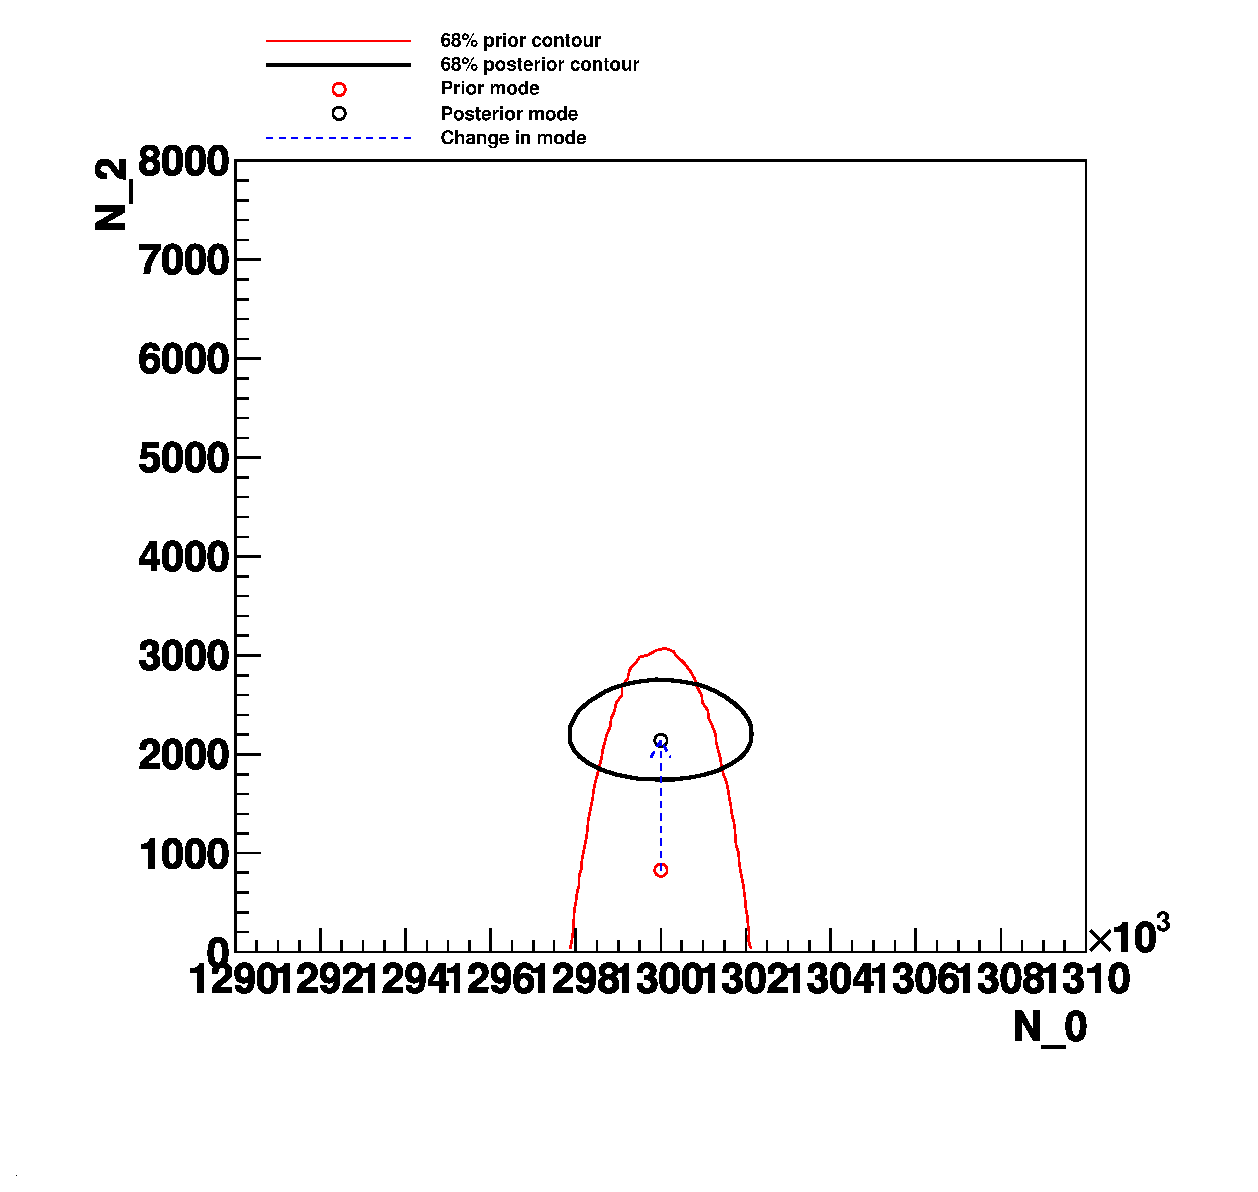
\includegraphics[width=0.45\textwidth]{./fig/lambda_fminus_vs_fbkg.eps}
\end{tabular}
\caption{Left: posterior probability for the parameter $\lambda_{+}$
(black line, denoted by N$_{3}$) and the prior probability (red
line). Right: Marginalized distribution of the parameters
$\lambda_{-}$ and $\lambda_{\mathrm{bkg}}$ (denoted by N$_{2}$ and
N$_{0}$, respectively) including the smallest region containing 68\%
of the probability (black contour). The red and black circles
represent the global mode before and after the fit, respectively.}
\label{fig:marg}
\end{center}
\end{figure}

\begin{comment}
\subsection{Ensemble tests}

The exercise was repeated with a varying fraction contribution of
$\lambda_{+}$. A total of 1,000 data sets were generated for each
setting, and the data was analyzed in the way described above.

Figures:
%
\begin{itemize}
\item chi2 and KS vs. $\lambda_{+}$,
\item fraction of discoveries vs. $\lambda_{+}$,
\item estimated $\lambda_{i}$ vs. $\lambda_{+}$ (simple model), 
\item estimated $\lambda_{i}$ vs. $\lambda_{+}$ (complex model), 
\item estimated $\lambda_{i}$ vs. $\lambda_{+}$ (mixed model), 
\item estimated (90\%) limit on $\lambda_{+}$ vs. $\lambda_{+}$, 
\end{itemize}

Conclusion. \\ 
\end{comment}

% -----------------------------------------------------
% implementation
% -----------------------------------------------------

\section{Technical implementation} 
\label{implementation}

The tool used for the analysis presented in this note is based
BAT~\cite{Caldwell:2008fw} and freely available on the web
page~\cite{BATwebpage}. An arbitrary number of templates can be used
to fit a data set. Efficiencies and uncertainties can be defined as a
function of the variable $x$ under study. Systematic uncertainties are
included as nuisance parameters following eqn.~\ref{eqn:syst}, i.e.,
Gaussian uncertainties can be defined individually for each
contribution. The global mode and the marginalized distributions are
extracted. Error bands on the contributions are calculated and plots
for the best-fit estimate are produced as that shown in
fig.~\ref{fig:stack}. The goodness-of-fit is tested using the
$\chi^{2}$ and the Kolmogorov-Smirnov tests as well as a
$p$-value. The tool comes with a machinery to perform automated
ensemble tests. Calibration curves and pull distributions are thus
easily accessible. \\

% -----------------------------------------------------
% bibliography 
% -----------------------------------------------------

\clearpage 
\pagebreak 

\begin{thebibliography}{99}
%\bibitem{Caldwell:2006yj}
%  A.~Caldwell and K.~Kr{\"o}ninger,
%  ``Signal discovery in sparse spectra: a Bayesian analysis,''
%  Phys.\ Rev.\  D {\bf 74} (2006) 092003
%  [arXiv:physics/0608249].
\bibitem{Caldwell:2008fw}
  A.~Caldwell, D.~Kollar and K.~Kr{\"o}ninger, \\ 
  ``BAT - The Bayesian Analysis Toolkit,'' \\ 
  Comput. Phys. Commun. {\bf 180} (2009) 2197 [arXiv:0808.2552]. 
\bibitem{BATwebpage}
  BAT can be found at the following url: \\ http://www.mppmu.mpg.de/bat/models/
\end{thebibliography} 

% -----------------------------------------------------

\end{document}


